% mycsrf 'for beeing included' snippet template
%
% (c) Karsten Reincke, Frankfurt a.M. 2012, ff.
%
% This text is licensed under the Creative Commons Attribution 3.0 Germany
% License (http://creativecommons.org/licenses/by/3.0/de/): Feel free to share
% (to copy, distribute and transmit) or to remix (to adapt) it, if you respect
% how you must attribute the work in the manner specified by the author(s):
% \newline
% In an internet based reuse please link the reused parts to mycsrf.fodina.de
% and mention the original author Karsten Reincke in a suitable manner. In a
% paper-like reuse please insert a short hint to mycsrf.fodina.de and to the
% original author, Karsten Reincke, into your preface. For normal quotations
% please use the scientific standard to cite
%


%% use all entries of the bibliography

\subsection{Brahms (-)}

\parpic(1cm,1cm)[r][t]{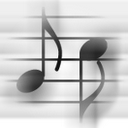
\includegraphics[width=1cm]{logos/brahms-300dpi.png}}
\label{Brahms}\acc{Wikipedia} zählt \acc{Brahms} zu den \enquote{Sequenzern},
die \enquote{[\ldots] neben ihrem Hauptanwendungsfeld der Audio- und
MIDI-Bearbeitung auch Notensatzfunktionalitäten
(beinhalten)}.\footcite[vgl.][\nopage wp]{WpedNotensatz2019a} Wir sind geneigt,
von 'Geistersoftware' zu sprechen:

Das Programm \acc{Brahms} wird in einer älteren Sichtung auf ein
Sourceforgeprojekt verlinkt\footcite[vgl.][\nopage wp]{Callon2009a}, in der
aktuelleren aber nicht.\footcite[vgl.][\nopage wp]{WpedNotensatz2019a}
Suchmaschinen beantworten den Request '\texttt{brahms musicsoftware}' im
Wesentlichen mit obigen Listen, deren Duplikate und dem
Sourceforgeprojekt.\footnote{$\rightarrow$
\href{https://www.google.com/search?q=brahms+musicsoftware}
{https://www.google.com/search?q=brahms+musicsoftware} (RDL 20190209)} Die
Homepage dieses \acc{Brahms-Sourceforge-Projektes} nutzt dann -- beruhigender-
und letztlich irreführenderweise -- ein Logo mit Noten.\footcite[vgl.][\nopage
wp]{Brahms2013a} Dennoch hat (dieses) \acc{Brahms} (von sich aus) nichts mit
Musik zu tun: es sei ein \enquote{[\ldots] Modular Execution Framework (MEF) for
executing integrated systems built from component software processes}, ein
\enquote{SystemML-ready execution client}.\footcite[vgl.][\nopage
wp]{Brahms2013b} Mittlerweile gibt es dazu ein neueres Github-Repository, das
per 'Fork' aus dem Sourceforgeprojekt entstanden ist. Und unter Github
beschreibt sich \acc{Brahms} -- direkt und ganz ohne Notenlogo -- als
\enquote{simulation execution engine}.\footcite[vgl.][\nopage wp]{Brahms2018a}

Tatsächlich ist (dieses) \acc{Brahms} kein Sequencer mit Notensatzfunktion. Und
wenn es solch ein Programm früher einmal gegeben hat -- wir vermuten eher, dass
das Logo und die Beschreibung frühere Begutachter in die Irre führte --, dann
sind die Repositories durcheinander geraten. Oder aber das richtige Notensatz-
und Sequencerprogramm \acc{Brahms} wird so versteckt gepflegt, dass auch der
unbedarfte Musikwissenschaftler es nicht einfach und schnell genug finden wird.
So läuft alles auf dasselbe hinaus: heute ist \acc{Brahms} in dieser Funktion
nicht nutzbar.


% this is only inserted to eject fault messages in texlipse
%\bibliography{../bib/literature}
